\documentclass[tikz,border=7pt]{standalone}

\usepackage{amsmath}
\usetikzlibrary{arrows.meta,backgrounds,calc,fit,positioning}

\definecolor{sourcedatablue}{HTML}{4C78A8}
\definecolor{targetorange}{HTML}{F28E2B}
\definecolor{modelpurple}{HTML}{8B6BB1}
\definecolor{predictiongreen}{HTML}{59A14F}
\definecolor{panelgray}{HTML}{8A8A8A}

\begin{document}
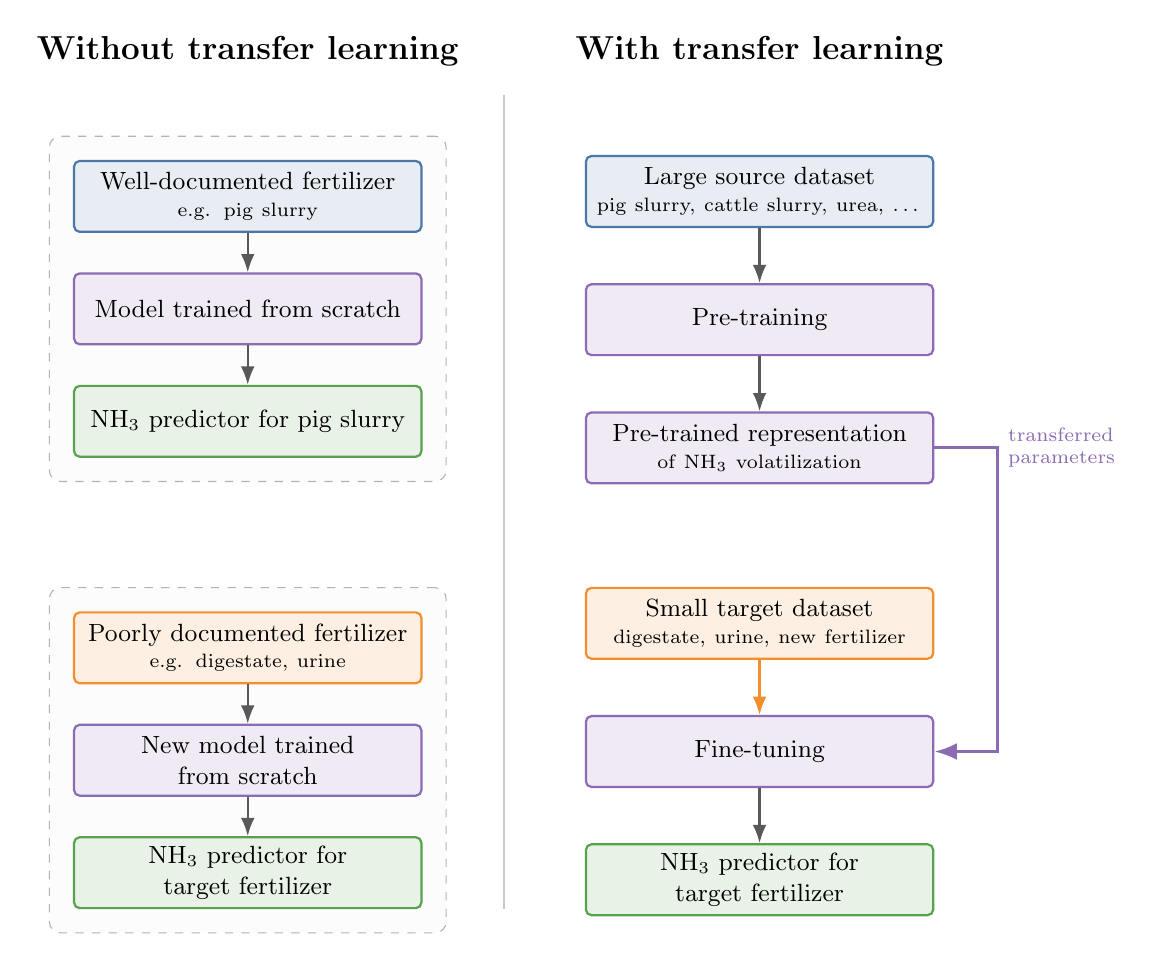
\begin{tikzpicture}[
  >=Latex,
  every node/.style={align=center},
  title/.style={font=\bfseries\large},
  subtitle/.style={font=\bfseries\scriptsize, text=black!65},
  box/.style={rectangle, rounded corners=2pt, draw, line width=0.8pt,
              text width=42mm, minimum height=9mm,
              inner sep=3pt, font=\small},
  source/.style={box, draw=sourcedatablue, fill=sourcedatablue!13},
  target/.style={box, draw=targetorange, fill=targetorange!14},
  model/.style={box, draw=modelpurple, fill=modelpurple!14},
  prediction/.style={box, draw=predictiongreen, fill=predictiongreen!14},
  flow/.style={->, draw=black!65, line width=0.8pt},
  transfer/.style={->, draw=modelpurple, line width=1.15pt},
  group/.style={rounded corners=4pt, draw=panelgray!65, dashed,
                fill=black!1, inner xsep=3mm, inner ysep=3mm}
]

% ------------------------------------------------------------------
% Without transfer learning: two independent configurations
% ------------------------------------------------------------------
\node[title] (left-title) at (0,0) {Without transfer learning};

\node[subtitle] (config-1) at (0,-0.85) {};
\node[source, below=4mm of config-1] (pig-data)
  {Well-documented fertilizer\\[-0.5mm]
   \scriptsize e.g. pig slurry};
\node[model, below=5mm of pig-data] (pig-model)
  {Model trained from scratch};
\node[prediction, below=5mm of pig-model] (pig-pred)
  {NH$_3$ predictor for pig slurry};

\draw[flow] (pig-data) -- (pig-model);
\draw[flow] (pig-model) -- (pig-pred);

\node[subtitle, below=13mm of pig-pred] (config-2) {};
\node[target, below=4mm of config-2] (target-data-left)
  {Poorly documented fertilizer\\[-0.5mm]
   \scriptsize e.g. digestate, urine};
\node[model, below=5mm of target-data-left] (target-model-left)
  {New model trained from scratch};
\node[prediction, below=5mm of target-model-left] (target-pred-left)
  {NH$_3$ predictor for target fertilizer};

\draw[flow] (target-data-left) -- (target-model-left);
\draw[flow] (target-model-left) -- (target-pred-left);

\begin{scope}[on background layer]
  \node[group, fit=(pig-data)(pig-model)(pig-pred)] {};
  \node[group, fit=(target-data-left)(target-model-left)
                   (target-pred-left)] {};
\end{scope}

% ------------------------------------------------------------------
% With transfer learning: source knowledge is adapted to a target task
% ------------------------------------------------------------------
\node[title] (right-title) at (6.5,0) {With transfer learning};

\node[source, below=10mm of right-title] (source-data)
  {Large source dataset\\[-0.5mm]
   \scriptsize pig slurry, cattle slurry, urea, \ldots};
\node[model, below=7mm of source-data] (pretrain) {Pre-training};
\node[model, below=7mm of pretrain] (representation)
  {Pre-trained representation\\[-0.5mm]
   \scriptsize of NH$_3$ volatilization};

\node[target, below=13mm of representation] (target-data-right)
  {Small target dataset\\[-0.5mm]
   \scriptsize digestate, urine, new fertilizer};
\node[model, below=7mm of target-data-right] (finetune) {Fine-tuning};
\node[prediction, below=7mm of finetune] (target-pred-right)
  {NH$_3$ predictor for target fertilizer};

\draw[flow] (source-data) -- (pretrain);
\draw[flow] (pretrain) -- (representation);
\draw[transfer] (representation.east) -- ++(0.8,0)
  node[right, font=\scriptsize, text=modelpurple, align=left]
  {transferred\\parameters} |- (finetune.east);
\draw[flow, draw=targetorange] (target-data-right) -- (finetune);
\draw[flow] (finetune) -- (target-pred-right);

% A subtle divider emphasizes the comparison between the two strategies.
\draw[panelgray!45, line width=0.7pt]
  (3.25,-0.55) -- ($(target-pred-left.south)+(3.25,0)$);

\end{tikzpicture}
\end{document}

